% ============================================================
% primer_avance.tex
% Primer avance del proyecto final (sintetizador musical).
% Solo diagramas de bloques, capturas de Quartus II 13.0 SP1 y
% salidas reales de los reportes y del programador.
% Compilar desde esta carpeta:  latexmk -pdf primer_avance.tex
% ============================================================
\documentclass[11pt]{article}
\usepackage[utf8]{inputenc}
\usepackage[T1]{fontenc}
\usepackage[spanish,es-noquoting]{babel}
\usepackage{lmodern}
\usepackage[a4paper,landscape,margin=1.6cm]{geometry}
\usepackage{graphicx}
\usepackage{booktabs}
\usepackage{float}
\usepackage{caption}
\usepackage{listings}
\usepackage{xcolor}
\usepackage{fancyhdr}
\usepackage[hidelinks]{hyperref}

\graphicspath{{../../capturas/}{../../docs/img/}}
\captionsetup{font=small,labelfont=bf}
\lstset{basicstyle=\ttfamily\footnotesize,columns=fullflexible,breaklines=true,
        frame=single,backgroundcolor=\color{gray!8}}

% ---- datos de la portada ----
\newcommand{\integrantes}{%
  Andrés Basilio Illescas\\
}
\newcommand{\repo}{https://github.com/samisal123/robot-seguidor-luz-vlsi}

\pagestyle{fancy}
\fancyhf{}
\lhead{\small Laboratorio de Diseño Digital VLSI}
\rhead{\small Proyecto final: sintetizador musical. Primer avance}
\cfoot{\small\thepage}

% una captura por pagina, lo mas grande posible
\newcommand{\captura}[2]{%
  \begin{figure}[H]
    \centering
    \includegraphics[width=\linewidth,height=0.76\textheight,keepaspectratio]{#1}
    \caption{#2}
  \end{figure}\clearpage}

\begin{document}

% ------------------------------------------------------------
\begin{titlepage}
  \centering
  {\large Universidad Nacional Autónoma de México\par}
  {\large Facultad de Ingeniería\par}
  \vspace{1.4cm}
  {\LARGE\bfseries Laboratorio de Diseño Digital VLSI\par}
  \vspace{0.8cm}
  {\Large Proyecto final: sintetizador musical\par}
  \vspace{0.3cm}
  {\Large Primer avance\par}
  \vspace{1.2cm}
  {\large \integrantes\par}
  \vspace{1.0cm}
  Tarjeta EP2C5T144 (Cyclone II EP2C5T144C8)\par
  Quartus II 13.0 SP1 Web Edition\par
  \vspace{0.3cm}
  Repositorio: \url{\repo}\par
  \vfill
  10 de noviembre de 2026
\end{titlepage}

% ------------------------------------------------------------
\section{Diagrama general de bloques}

\begin{figure}[H]
  \centering
  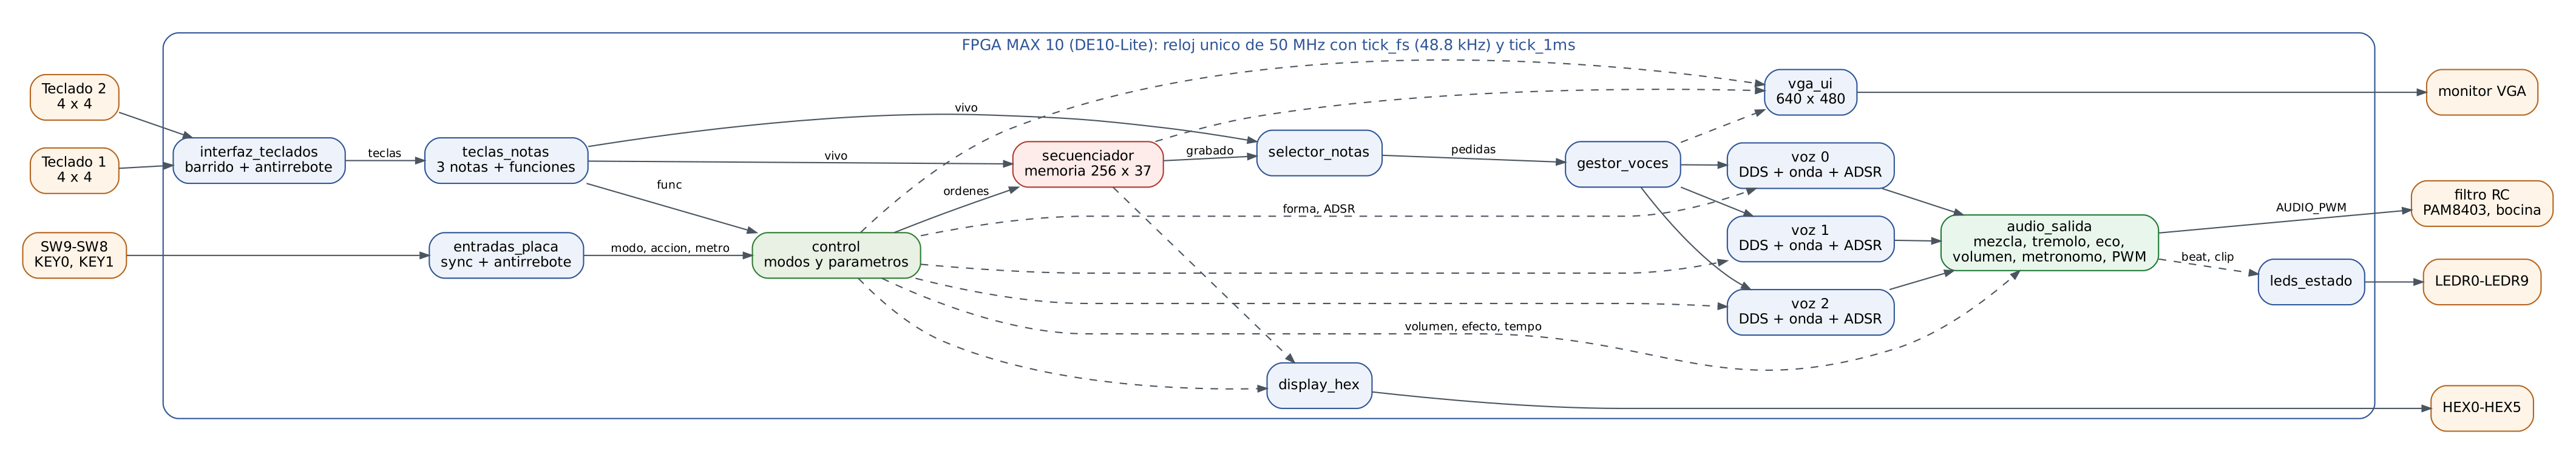
\includegraphics[width=\linewidth]{bloques.png}
  \caption{Diagrama general de bloques del sintetizador en la Cyclone II.}
\end{figure}
\clearpage

% ------------------------------------------------------------
\section{Proyecto en Quartus}

\captura{01_proyecto.png}{Proyecto en Quartus II 13.0 SP1 para la EP2C5T144C8 (pestaña Files).}
\captura{02_simbolo.png}{Creación del símbolo a partir del archivo .vhd (File, Create / Update, Create Symbol Files for Current File).}
\captura{06_top_level.png}{Jerarquía del proyecto con el diagrama de bloques \texttt{sintetizador} como nivel superior.}

% ------------------------------------------------------------
\section{Diagrama de bloques en Quartus}

\captura{03_bdf_completo.png}{Diagrama de bloques del sintetizador (\texttt{sintetizador.bdf}, nivel superior).}
\captura{05_bdf_control.png}{Mitad izquierda: reloj, reset, botones, teclados, control, secuenciador y selector de notas.}
\captura{04_bdf_voces.png}{Mitad derecha: gestor de voces, las 3 voces, salida de audio, VGA y LEDs.}
\captura{14_simbolos.png}{Símbolos de los módulos con sus puertos.}

% ------------------------------------------------------------
\section{Máquina de estados}

\captura{12_fsm_adsr.png}{Máquina de estados del ADSR de cada voz (State Machine Viewer).}

% ------------------------------------------------------------
\section{Compilación}

\begin{table}[H]
  \centering
  \caption{Resumen de la compilación (Flow Summary de Quartus y TimeQuest, modelo lento).}
  \begin{tabular}{ll}
    \toprule
    Concepto & Valor \\
    \midrule
    Dispositivo & EP2C5T144C8 (Cyclone II) \\
    Elementos lógicos & 3\,782 de 4\,608 (82\,\%) \\
    Funciones combinacionales & 3\,631 de 4\,608 (79\,\%) \\
    Registros & 1\,403 de 4\,608 (30\,\%) \\
    Bits de memoria & 76\,032 de 119\,808 (63\,\%) \\
    Multiplicadores de 9 bits & 6 de 26 (23\,\%) \\
    PLL & 1 de 2 \\
    Pines & 30 de 89 (34\,\%) \\
    Reloj del diseño & 25 MHz (PLL a partir de 50 MHz) \\
    Fmax & 36.05 MHz \\
    Holgura de setup / hold & 12.261 ns / 0.499 ns \\
    \bottomrule
  \end{tabular}
\end{table}
\clearpage

\captura{07_flow_summary.png}{Resumen de la compilación (Flow Summary).}
\captura{08_recursos_entidad.png}{Recursos por módulo (Fitter, Resource Utilization by Entity).}
\captura{10_fmax.png}{Frecuencia máxima (TimeQuest, Slow Model, Fmax Summary).}
\captura{11_rtl_viewer.png}{Vista RTL del nivel superior.}
\captura{09_pin_planner.png}{Asignación de pines (Pin Planner).}

% ------------------------------------------------------------
\section{Programación de la tarjeta}

La tarjeta se programó por JTAG con el USB-Blaster. Salida del programador de Quartus (sin los avisos de licencia):

\lstinputlisting[firstline=5]{../../logs/programacion_tarjeta.log}

\end{document}
